% !TeX spellcheck = en_US
\documentclass{beamer}

% --- Theme and Colors ---
\usetheme{Madrid}
\usecolortheme{default} % You can try others like "whale", "beaver", "orchid"

% --- Essential Packages ---
\usepackage[T1]{fontenc}
\usepackage[english]{babel}
\usepackage[utf8]{inputenc}
\usepackage{adjustbox}
\usepackage{lmodern}
\usepackage{graphicx}
\usepackage{xcolor}
\usepackage{amsmath, amssymb}
\usepackage{booktabs} % For nice tables
\usepackage{hyperref}
\usepackage{tikz}
\usepackage{fontawesome5} % For icons
\usepackage{multicol} % For multi-column layouts
\usepackage{listings} % For code snippets

% --- TikZ Libraries ---
\usetikzlibrary{shapes.geometric, arrows.meta, positioning, calc, mindmap, trees}

% --- Custom Commands ---
% Full-page image slide
\newcommand{\fullPageImage}[3]{%
  \begin{frame}[plain]
    \centering
    \begin{tikzpicture}[remember picture, overlay]
      \node[anchor=north, font=\LARGE\bfseries, text width=\paperwidth, align=center, yshift=-0.5cm] at (current page.north) {#1};
      \node[anchor=center] at (current page.center) {
        \includegraphics[width=0.85\paperwidth, height=0.75\paperheight, keepaspectratio]{#2}
      };
      \node[anchor=south east, font=\fontsize{8}{10}\selectfont, xshift=-0.5cm, yshift=0.5cm] at (current page.south east) {#3};
    \end{tikzpicture}
  \end{frame}
}

% --- Project Variables ---
\def\projectTitle{Neuroevolution-Based Game Bot for T-Rex Runner}
\def\projectSubtitle{Applying NEAT and Comparing with DDPG \& PPO}
\def\authorA{J. Chenye} % Replace with actual names
\def\authorB{W. Shaoyan}
\def\authorC{W. Xiaoxu}
\def\authorD{Q. Yonghui and W. Haoran}
\def\supervisorName{Dr. Syed Muhammad Abrar Akber \& Sadia Nishat Kazmi}
\def\courseName{Biologically Inspired Artificial Intelligence}
\def\university{Yanshan University \& Silesian University of Technology}
\def\locationDate{Qinhuangdao / Gliwice, May 2025} % Update year

% --- Presentation Info ---
\title{\projectTitle}
\subtitle{\projectSubtitle}
\author{\authorA \and \authorB \and \authorC \and \authorD}
\institute{\university}
\date{\locationDate}

% --- Logo ---
% \logo{
\includegraphics[height=0.7cm]{media/ysu.png}\hspace{0.5cm}\includegraphics[height=0.7cm]{media/sut_logo.png}} % Add SUT logo if available

% --- Listings Configuration for Python Code ---
\lstdefinestyle{pythoncode}{
  language=Python,
  basicstyle=\ttfamily\tiny, % Small font size for better fitting
  keywordstyle=\color{blue}\bfseries,
  commentstyle=\color{green!60!black},
  stringstyle=\color{orange},
  showstringspaces=false,
  numbers=left,
  numberstyle=\tiny\color{gray},
  breaklines=true,
  breakatwhitespace=true,
  tabsize=2,
  captionpos=b, % caption below
  frame=tb, % top and bottom frame lines
  emph={eval_genomes, TRexGame, neat, DDPGAgent, PPOAgent, step, reset}, % Custom keywords
  emphstyle=\color{purple}\bfseries
}


% --- Document Content ---
\begin{document}

% --- Title Page ---
{
  \setbeamertemplate{headline}{}
  \setbeamertemplate{footline}{}
  \begin{frame}[plain]
    \titlepage
    \begin{center}
      \vspace{0.5cm}
      
\includegraphics[height=1cm]{media/ysu.png} % Replace with actual YSU logo
      % \includegraphics[height=1cm]{media/sut_logo.png} % Replace with actual SUT logo
    \end{center}
  \end{frame}
}

% --- Outline ---
\begin{frame}{Table of Contents}
  \tableofcontents
\end{frame}

% --- Sections ---
\section{Introduction}

\begin{frame}{Authors' Contributions}
\begin{block}{Overview}
The following table summarizes the main contributions of each team member to the project:
\end{block}

\vspace{0.3cm}

\begin{table}[h!]
  \centering
  \scalebox{0.85}{
    \begin{tabular}{l|p{9cm}}
    \toprule
    \textbf{Author} & \textbf{Contribution} \\
    \midrule
    Jin Chenye & 30\% Write NEAT code, front-end code, and AI explainability exploration, network evolution video (with ffmpeg) \\
    Wang Shaoyan & 30\% Write PPO, DDPG code, modify game code, and conceive artificial intelligence network design. \\
    Wang Xiaoxu & 15\% Design of PPO network, conception of NEAT artificial intelligence network design, and summary of achievements. \\
    Qi Yonghui & 15\% Design of DDPG network, conception of NEAT artificial intelligence network design, and summary of achievements. \\
    Wu Haoran & 10\% Conceived NEAT artificial intelligence network design, and proposed comparative ideas. \\
    \bottomrule
    \end{tabular}
  }
\end{table}
\end{frame}


\begin{frame}{Project Overview: T-Rex Runner Automation}
  \begin{columns}[T]
    \begin{column}{0.6\textwidth}
      \begin{block}{Project Goal}
        To develop an intelligent agent capable of playing the Chrome T-Rex Runner game autonomously using biologically inspired AI techniques, primarily NeuroEvolution of Augmenting Topologies (NEAT).
      \end{block}
    \end{column}
    \begin{column}{0.4\textwidth}
      \centering
      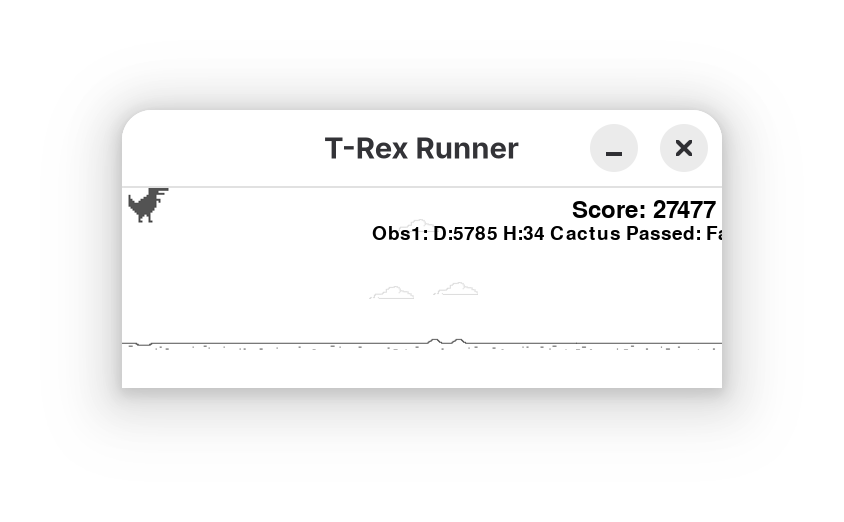
\includegraphics[width=\linewidth]{media/trex_game.png} % Screenshot of T-Rex game
      \tiny T-Rex Runner Game Interface
    \end{column}
  \end{columns}
  \begin{block}{Motivation}
        \begin{itemize}
          \item Explore the capabilities of neuroevolution in dynamic game environments.
          \item Understand the process of designing fitness functions for evolutionary algorithms.
          \item Compare NEAT's performance against other Reinforcement Learning (RL) methods like DDPG and PPO.
        \end{itemize}
      \end{block}
\end{frame}

\begin{frame}{Project Requirements}
  This project aligns with "Project 3: Neuroevolution-Based Game Bot".
  \begin{block}{Core Requirements Met}
    \begin{itemize}
      \item Create a simple game-playing bot (T-Rex Runner instead of Flappy Bird).
      \item Bot learns by evolving its neural network (brain) over time.
      \item Observe bot improvement over generations.
      \item Recommended Tools: Python, Pygame, NEAT-Python.
    \end{itemize}
  \end{block}
  \begin{block}{Output Requirements Met}
    \begin{itemize}
      \item \faCheck~ Functional game bot that learns to play.
      \item \faCheck~ Training performance curve showing improvement.
      \item \faCheck~ Video recording or GIF of gameplay (planned for demo).
      \item \faCheck~ Well-structured code using NEAT-Python.
      \item \textit{Bonus:} Comparison with DDPG and PPO, detailed analysis of training.
    \end{itemize}
  \end{block}
\end{frame}

\section{Background: Biologically Inspired AI}

\begin{frame}{NeuroEvolution of Augmenting Topologies (NEAT)}
  \begin{block}{What is NEAT?}
    A sophisticated GA that evolves not only the weights of a neural network but also its topology (structure).
    \begin{itemize}
        \item \textbf{Starts Minimal:} Begins with simple networks and gradually adds complexity (nodes and connections).
        \item \textbf{Historical Markings (Innovation Numbers):} Tracks gene origins to solve the "competing conventions" problem in crossover. Allows meaningful crossover between different topologies.
        \item \textbf{Speciation:} Divides the population into species based on topological similarity. Protects innovation by allowing new structures time to optimize within their own niche.
    \end{itemize}
  \end{block}
  \begin{figure}
      \centering
      % Simple diagram of NEAT adding a node and a connection
      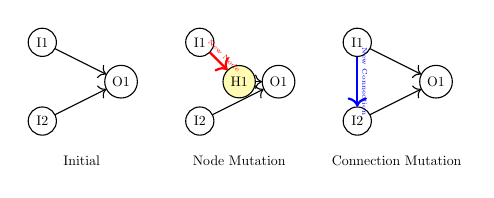
\begin{tikzpicture}[scale=0.5, every node/.style={transform shape}]
          \node[circle, draw, minimum size=0.5cm] (i1) at (0,1) {I1};
          \node[circle, draw, minimum size=0.5cm] (i2) at (0,-1) {I2};
          \node[circle, draw, minimum size=0.5cm] (o1) at (2,0) {O1};
          \draw[->] (i1) -- (o1);
          \draw[->] (i2) -- (o1);
          \node at (1,-2) {Initial};

          \node[circle, draw, minimum size=0.5cm] (i1b) at (4,1) {I1};
          \node[circle, draw, minimum size=0.5cm] (i2b) at (4,-1) {I2};
          \node[circle, draw, fill=yellow!30, minimum size=0.5cm] (h1) at (5,0) {H1};
          \node[circle, draw, minimum size=0.5cm] (o1b) at (6,0) {O1};
          \draw[->,red,thick] (i1b) -- (h1) node[midway,above,sloped,font=\tiny,color=red] {New Node};
          \draw[->] (h1) -- (o1b);
          \draw[->] (i2b) -- (o1b);
          \node at (5,-2) {Node Mutation};

          \node[circle, draw, minimum size=0.5cm] (i1c) at (8,1) {I1};
          \node[circle, draw, minimum size=0.5cm] (i2c) at (8,-1) {I2};
          \node[circle, draw, minimum size=0.5cm] (o1c) at (10,0) {O1};
          \draw[->] (i1c) -- (o1c);
          \draw[->,blue,thick] (i1c) -- (i2c) node[midway,above,sloped,font=\tiny,color=blue] {New Connection};
          \draw[->] (i2c) -- (o1c);
          \node at (9,-2) {Connection Mutation};
      \end{tikzpicture}
      \caption{NEAT evolves network topology.}
  \end{figure}
\end{frame}

\section{Methodology}

\begin{frame}{The T-Rex Runner Game Environment}
  \begin{columns}[T]
    \begin{column}{0.5\textwidth}
      \begin{block}{Environment (`aiGame.py`)}
        \begin{itemize}
            \item Implemented using \textbf{Pygame}.
            \item Player (T-Rex) must avoid cacti and birds.
            \item Game speed gradually increases.
            \item Provides state information to the agent and receives actions.
        \end{itemize}
      \end{block}
      \begin{block}{Key Features}
          \begin{itemize}
              \item Obstacle generation logic.
              \item Collision detection.
              \item Scoring mechanism.
              \item Player can: Jump, Duck, No-op.
          \end{itemize}
      \end{block}
    \end{column}
    \begin{column}{0.5\textwidth}
      \centering
      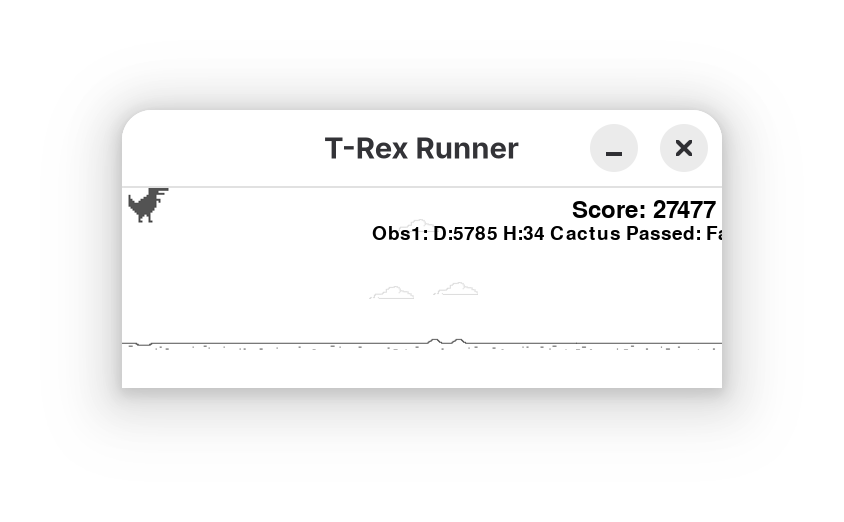
\includegraphics[width=\linewidth]{media/trex_game.png} \\
      
\includegraphics[width=0.9\linewidth]{media/resources.png} \\ % Snippet of resources.png
      \tiny Game Sprites from `resources.png`
    \end{column}
  \end{columns}
\end{frame}

\begin{frame}{State Representation \& Action Space (NEAT)}
  \begin{block}{State Vector (Inputs to Neural Network)}
    The environment provides a 14-dimensional state vector, normalized for better NN performance:
    \begin{enumerate}
        \item Player Y position
        \item Player vertical velocity
        \item Is crouching (binary)
        \item Obstacle 1: X distance
        \item Obstacle 1: Y position
        \item Obstacle 1: Width
        \item Obstacle 1: Height
        \item Obstacle 1: Is bird (binary)
    \end{enumerate}
    \tiny (Normalization details in `DDPG\_train.py` and `PPO\_train.py`, applied consistently for NEAT)
  \end{block}
\end{frame}

\begin{frame}{State Representation \& Action Space (NEAT)}
  \begin{block}{Action Space (Outputs from Neural Network)}
    The NEAT network outputs scores for 3 discrete actions:
    \begin{itemize}
        \item \textbf{Action 0}: No-op (continue running)
        \item \textbf{Action 1}: Jump
        \item \textbf{Action 2}: Duck / Fast-fall (if already jumping)
    \end{itemize}
    The action with the highest output score is chosen.
  \end{block}
\end{frame}

\begin{frame}{Fitness Function Design (NEAT) - \textit{Highlight}}
  The fitness function is crucial for guiding evolution. Our design:
  \begin{block}{Base Fitness Components}
    \begin{itemize}
        \item \textbf{Survival Reward}: `+0.1` for each game tick the T-Rex survives. Encourages longevity.
        \item \textbf{Obstacle Pass Reward}: `+10` for successfully passing an obstacle. Encourages progress.
        \item \textbf{Crash Penalty}: `-1` (implicitly, as game ends and fitness accumulation stops, also a fixed penalty can be added). Discourages dying.
    \end{itemize}
  \end{block}
\end{frame}

% \begin{frame}{Fitness Function Design (NEAT) - \textit{Highlight}}
%   \begin{block}{Strategic Bird Penalty/Reward (`bird\_penalty`) - \textit{Key Innovation}}
%     To encourage intelligent behavior against birds, a penalty/reward system was added:
%     \begin{itemize}
%         \item Applied when T-Rex is close to a bird (`abs(obs1\_dist\_x) < overlap\_threshold`).
%         \item \textbf{High-flying bird (should duck):}
%         \begin{itemize}
%             \item Jump: `-20` (strong penalty for wrong action)
%             \item No-op: `-10` (penalty for inaction)
%             \item Duck: `+0` (correct action, no penalty)
%         \end{itemize}
%         \item \textbf{Low-flying bird (should jump):}
%         \begin{itemize}
%             \item Duck: `-20`
%             \item No-op: `-10`
%             \item Jump: `+0`
%         \end{itemize}
%         \item \textbf{Mid-height bird (either duck or jump is fine):}
%         \begin{itemize}
%             \item No-op: `-10` (penalty for inaction if an action could be beneficial)
%         \end{itemize}
%     \end{itemize}
%     \textit{Rationale: This guides the agent in learning context-specific actions for different bird altitudes, significantly improving performance beyond simple survival.}
% \end{block}
% \end{frame}

\begin{frame}[fragile] % Use fragile for verbatim content
    \frametitle{Bird Penalty Logic in \texttt{eval\_genomes}}
    \begin{lstlisting}[
        style=pythoncode,
        caption={Excerpt from `NEAT/train\_neat.py` showing the bird penalty logic.}
    ]
# state, reward, done = game.step(action)
# fitness += reward # Original part
bird_penalty = 0
overlap_threshold = 5 + (state["obs1_width"] if state["obs1_is_bird"] else 0)

if state["obs1_is_bird"] and (abs(state["obs1_dist_x"]) < overlap_threshold):
    bird_y = state["obs1_y"]
    if bird_y <= 85:  # High-flying bird (should duck)
        if action == 1: bird_penalty -= 20 # Penalty for jumping
        elif action == 0: bird_penalty -= 10 # Penalty for no-op
        # elif action == 2: bird_penalty += 0 # Correct action (duck)
    elif bird_y >= 125:  # Low-flying bird (should jump)
        if action == 2: bird_penalty -= 20 # Penalty for ducking
        elif action == 0: bird_penalty -= 10 # Penalty for no-op
        # elif action == 1: bird_penalty += 0 # Correct action (jump)
    else:  # Mid-height bird
        if action == 0: bird_penalty -= 10 # Penalty for no-op if action is better

state, reward, done = game.step(action) # Action performed AFTER penalty logic
fitness += reward + bird_penalty # Add bird penalty to fitness
    \end{lstlisting}
\end{frame}

\begin{frame}{NEAT Training Process \& Seed Strategy - \textit{Highlight}}
  \begin{block}{NEAT Configuration (`neat-config.txt`)}
    \begin{itemize}
        \item Defines population size, fitness thresholds, mutation rates, speciation parameters, etc.
        \item Key parameters:
            \begin{itemize}
                \item `pop\_size = 100`
                \item `fitness\_criterion = mean`
                \item `num\_inputs = 14`, `num\_outputs = 3`
                \item Various mutation probabilities (node, connection, weight).
            \end{itemize}
    \end{itemize}
  \end{block}
\end{frame}

\begin{frame}{NEAT Training Process \& Seed Strategy - \textit{Highlight}}
  \begin{block}{Training Loop (`train\_neat.py`)}
    \begin{itemize}
        \item Iterates for a specified number of generations.
        \item In each generation, `eval\_genomes` evaluates all genomes.
        \item NEAT library handles selection, crossover, mutation, and speciation.
        \item Checkpoints and best genomes are saved periodically and on new best fitness.
        \item Detailed statistics (best/avg/std fitness, species count, genome complexity) are logged and saved.
    \end{itemize}
  \end{block}
\end{frame}

\begin{frame}{NEAT Training Process \& Seed Strategy - \textit{Highlight}}
  \begin{block}{Seed Strategy - \textit{Key for Reproducibility \& Exploration}}
    A two-phase seed strategy was implemented:
    \begin{itemize}
        \item \textbf{Phase 1 (Fixed Seed):} For the initial `fixed\_seed\_generations` (e.g., first 100-200 generations) OR until a `min\_fitness\_for\_random` (e.g., 3000) is achieved.
            \begin{itemize}
                \item \textit{Purpose:} Provides a consistent environment for early learning, allowing promising basic structures to emerge without being overly penalized by random difficult game sequences. Helps in comparing initial learning trajectories.
            \end{itemize}
        \item \textbf{Phase 2 (Random Seed):} After the conditions for Phase 1 are met.
            \begin{itemize}
                \item \textit{Purpose:} Exposes the evolving agents to a wider variety of game scenarios, promoting robustness and generalization. Prevents overfitting to a single game seed.
            \end{itemize}
    \end{itemize}
  \end{block}
\end{frame}

\begin{frame}{DDPG and PPO for Benchmarking}
To compare NEAT with mainstream DRL methods, DDPG and PPO were adapted to the T-Rex game:
\begin{columns}[T]
  \begin{column}{0.5\textwidth}
    \begin{block}{DDPG}
      \begin{itemize}
          \item Actor-critic, model-free.
          \item Adapted for discrete actions (Gumbel-Softmax).
          \item Replay buffer + target networks.
          \item Files: \texttt{DDPG/DDPG\_agent.py}
      \end{itemize}
    \end{block}
  \end{column}
  \begin{column}{0.5\textwidth}
    \begin{block}{PPO}
      \begin{itemize}
          \item Actor-critic, model-free.
          \item Clipped surrogate objective for stable updates.
          \item Batching experience updates.
          \item Files: \texttt{PPO/ppo\_agent.py}
      \end{itemize}
    \end{block}
  \end{column}
\end{columns}

\vspace{0.3cm}
\begin{block}{Common Features}
\begin{itemize}
  \item Use same 14-dim state as NEAT.
  \item Output discrete actions (0, 1, 2).
  \item Trained in the same environment.
\end{itemize}
\end{block}
\end{frame}



\section{Implementation Details}

\begin{frame}[fragile]{Project Directory Structure}
  \begin{tiny} % Use tiny font for the verbatim block to save space
    \begin{verbatim}
.
├── DDPG/
│   ├── aiGame.py
│   ├── DDPG_agent.py
│   └── DDPG_train.py
├── NEAT/  (Primary Focus)
│   ├── aiGame.py (T-Rex Environment)
│   ├── neat-config.txt (NEAT Parameters)
│   ├── train_neat.py (Training Script)
│   ├── play_trex_neat.py (Run Best Agent)
│   ├── visualize.py (Network Plotting)
│   ├── server.py (Web Visualization Interface)
│   ├── saved_models/ (Checkpoints, Genomes, Stats)
│   │   ├── neat-checkpoint-X
│   │   ├── neat-best-genome-overall.pkl
│   │   └── neat_stats_data.pkl
│   └── resources.png (Game Assets)
├── PPO/
│   ├── aiGame.py
│   ├── ppo_agent.py
│   └── ppo_train.py
└── ... (Other files like LICENSE)
    \end{verbatim}
  \end{tiny}
\end{frame}

\begin{frame}{Challenges \& Solutions}
    \begin{block}{Challenge 1: Slow Initial Learning / Stagnation}
        \begin{itemize}
            \item \textbf{Problem:} Agents struggled to learn basic survival or make meaningful progress.
            \item \textbf{Solution:}
                \begin{itemize}
                    \item \textit{Refined Fitness Function:} Added specific rewards for passing obstacles and the strategic bird penalty to guide learning more effectively.
                    \item \textit{Seed Strategy:} Used fixed seed initially to provide a consistent learning environment, reducing early randomness.
                \end{itemize}
        \end{itemize}
    \end{block}
    \pause
    \begin{block}{Challenge 2: Optimal Action Against Birds}
        \begin{itemize}
            \item \textbf{Problem:} Agents often failed to distinguish between high and low birds, leading to suboptimal actions (e.g., jumping into a high bird).
            \item \textbf{Solution:} The `bird\_penalty` system in the fitness function directly addresses this by penalizing incorrect actions based on bird altitude.
        \end{itemize}
    \end{block}
\end{frame}

\begin{frame}{Challenges \& Solutions}
    \begin{block}{Challenge 3: Long Training Times \& Resource Management}
        \begin{itemize}
            \item \textbf{Problem:} NEAT can be computationally intensive, requiring many generations.
            \item \textbf{Solution:}
                \begin{itemize}
                    \item Implemented robust checkpointing to resume training.
                    \item Optimized `aiGame.py` for faster simulation where possible.
                    \item Focused fitness function to accelerate learning of crucial behaviors.
                \end{itemize}
        \end{itemize}
    \end{block}
\end{frame}

\section{Results and Analysis}

\begin{frame}{NEAT Training Performance}
  \begin{columns}[T]
    \begin{column}{0.65\textwidth}
      \centering
      % Assuming 'neat_custom_fitness_curve.png' is the correct file
      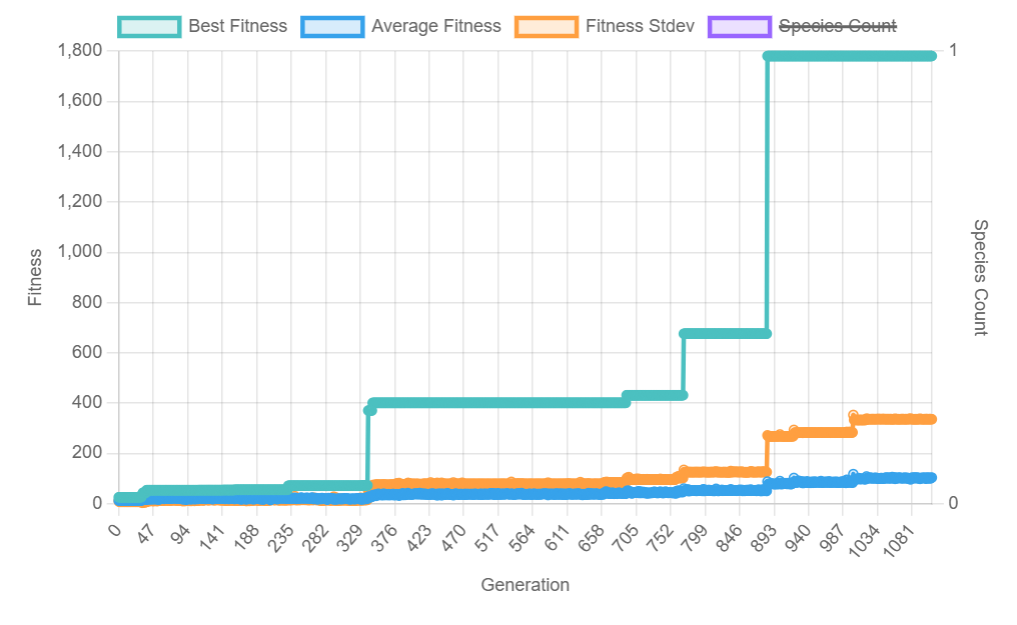
\includegraphics[width=\linewidth]{media/neat_custom_fitness_curve.png}
      \tiny Best, Average, and Std Dev Fitness over Generations.
    \end{column}
    \begin{column}{0.35\textwidth}
      \begin{block}{Observations}
        \begin{itemize}
            \item Steady increase in best fitness.
            \item Average fitness also shows upward trend.
            \item Standard deviation indicates diversity in population.
            \item Note periods of stagnation followed by breakthroughs (typical of EAs).
            \item (Mention when seed strategy switched if visible effect).
        \end{itemize}
      \end{block}
    \end{column}
  \end{columns}
\end{frame}

\begin{frame}{NEAT Speciation and Genome Complexity}
  \begin{columns}[T]
    \begin{column}{0.5\textwidth}
      \centering
      % Assuming 'neat\_species\_count.png' is the correct file
      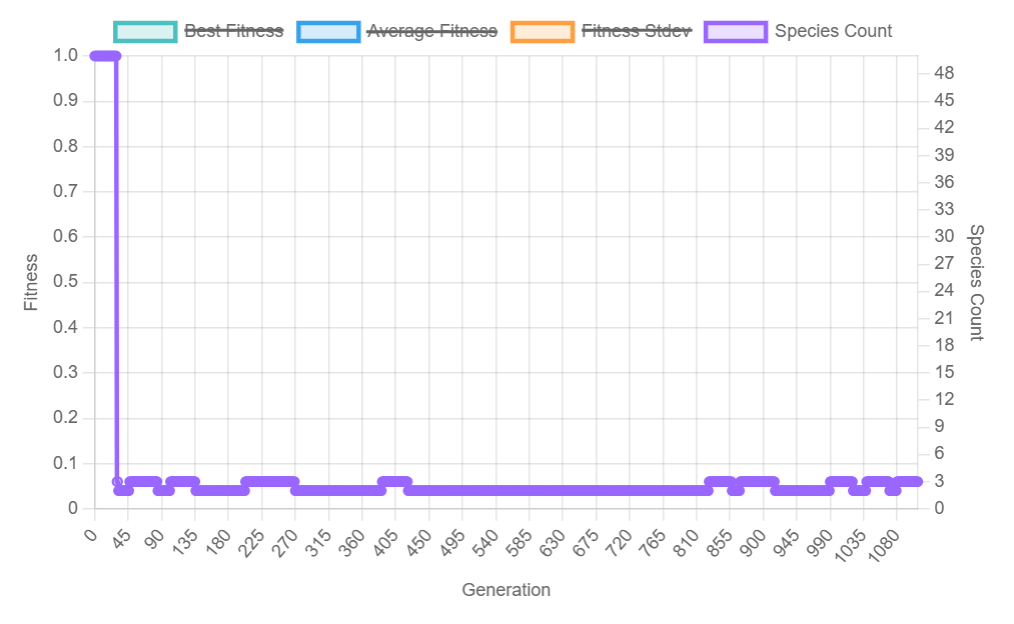
\includegraphics[width=\linewidth]{media/neat_species_count.jpg}
      \tiny Number of Species Over Generations.
      \begin{itemize}
        \item Shows dynamic nature of speciation.
        \item New species emerge, some die out.
        \item Helps protect innovation.
      \end{itemize}
    \end{column}
    \begin{column}{0.5\textwidth}
      \centering
      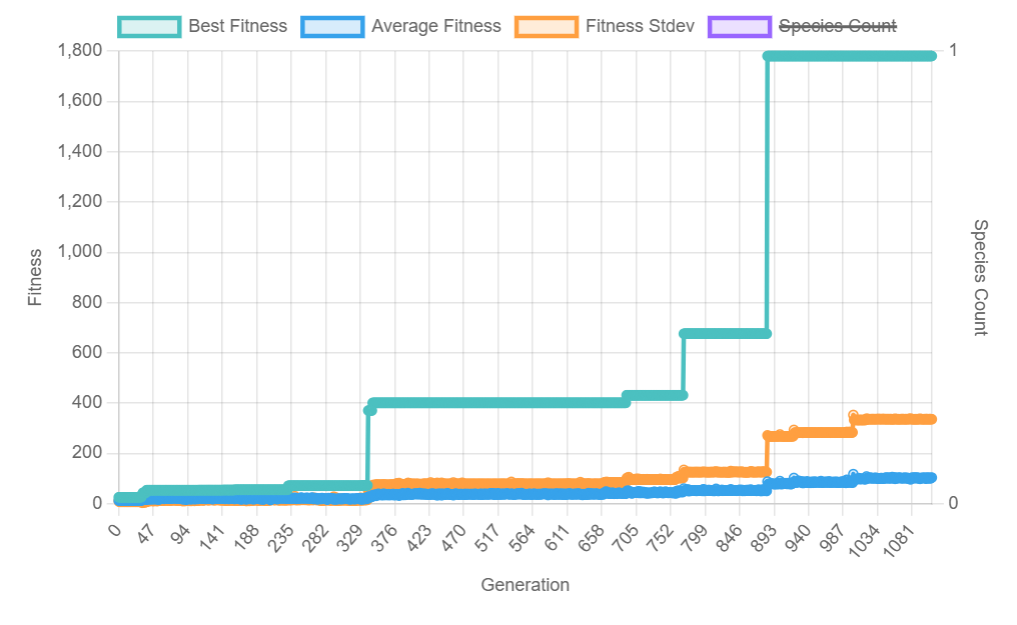
\includegraphics[width=\linewidth]{media/neat_genome_complexity.png}
      \tiny Complexity (Nodes \& Connections) of Best Genome.
      \begin{itemize}
        \item Generally, complexity increases over time as NEAT finds more sophisticated solutions.
      \end{itemize}
    \end{column}
  \end{columns}
\end{frame}

% --- BEGIN NEW SLIDE ---
\begin{frame}{Further Insights into NEAT Evolution}
\scalebox{0.75}{
\begin{minipage}{1.33\textwidth}  % 1 / 0.75 ≈ 1.33 to compensate width shrink
    \begin{block}{Network Evolution Trends}
        Observations from analyzing training process videos (e.g., `complexity\_evolution.mp4`, `fitness\_evolution.mp4`, `network\_rankX\_evolution.mp4`):
        \begin{itemize}
            \item Network evolution primarily converged towards two main structural directions, often based around specific persistent hidden nodes (e.g., nodes analogous to 47 and 12 in certain successful lineages).
            \item The fitness distribution among the population tended to become more uniform over extended training, indicating a convergence towards high-performing solutions or niches.
        \end{itemize}
    \end{block}
    \begin{block}{Genome Complexity Observations}
        \begin{itemize}
            \item Genome complexity (number of nodes and connections) for high-performing individuals often stabilized within a range of approximately 5-12 nodes and 15-23 connections.
            \item There wasn't always a strong direct correlation between higher complexity and higher fitness in later stages; effective, relatively simpler structures often persisted.
        \end{itemize}
    \end{block}
    \tiny \textit{These insights are based on detailed analysis of recorded training data and videos.}
\end{minipage}
}
\end{frame}

% --- END NEW SLIDE ---

% --- BEGIN NEW SLIDE ---
\begin{frame}{Key Moments in Training Evolution}
    \begin{block}{"Cretaceous Extinction" Event (Generations ~29-30)}
        \begin{itemize}
            \item Around generations 29-30, a significant reduction in species diversity was observed.
            \item This suggests a period where many less-fit genetic lines were unable to adapt and died out, a sort of "survival of the fittest" bottleneck.
            \item This evolutionary pressure likely paved the way for more robust strategies to emerge from the surviving species.
        \end{itemize}
    \end{block}
    \pause
    \begin{block}{The "Aha Moment" (Generations ~246-247)}
        \begin{itemize}
            \item A dramatic jump in maximum fitness occurred between generations 246 and 247.
            \item The average fitness also showed a corresponding oscillating increase.
            \item Analysis revealed that at this point, the agent learned to overcome a specific, previously insurmountable small cactus obstacle. This breakthrough represents a critical learning milestone.
        \end{itemize}
    \end{block}
    \tiny \textit{These events highlight the dynamic and punctuated nature of evolutionary learning.}
\end{frame}
% --- END NEW SLIDE ---

% --- BEGIN NEW SLIDE ---
\begin{frame}{The 'Aha Moment': Conquering a Critical Obstacle (Gen 246 vs. 247)}
    \begin{columns}[T]
        \begin{column}{0.5\textwidth}
            \centering
            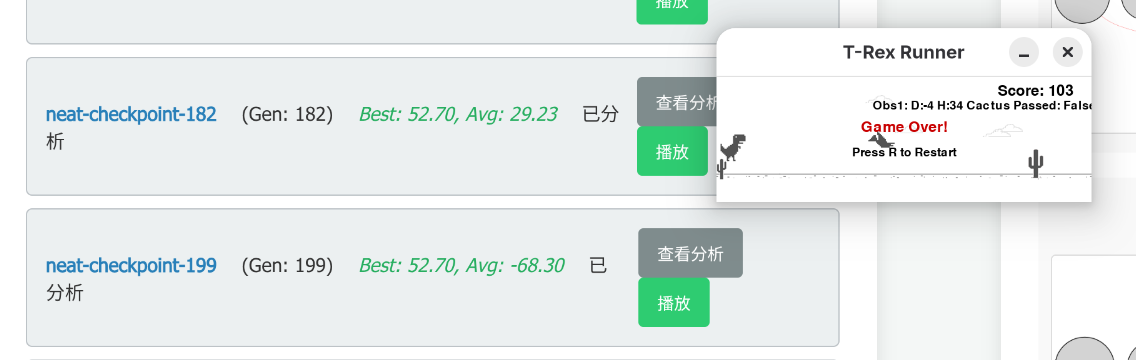
\includegraphics[width=0.9\linewidth]{media/gen246_stuck_cactus.png} % REPLACE with your Gen 246 image
            \tiny \textbf{Generation 246:} Agent consistently fails at this specific small cactus.
        \end{column}
        \begin{column}{0.5\textwidth}
            \centering
            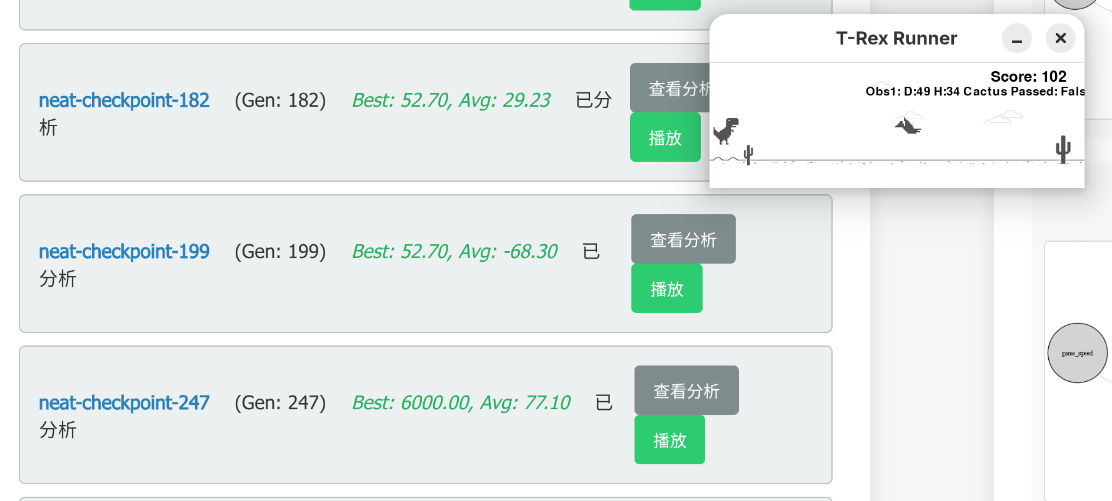
\includegraphics[width=0.9\linewidth]{media/gen247_pass_cactus.png} % REPLACE with your Gen 247 image
            \tiny \textbf{Generation 247:} Agent successfully learns to navigate the same obstacle.
        \end{column}
    \end{columns}
    \vspace{0.5cm}
    \begin{block}{Significance}
        This transition clearly demonstrates a specific learning event where the evolutionary process discovered a strategy (likely a subtle change in network weights or topology) to overcome a persistent challenge, leading to a significant performance boost.
    \end{block}
\end{frame}
% --- END NEW SLIDE ---


\begin{frame}{Analysis of Best Evolved NEAT Agent}
      \centering
      \begin{figure}
          \centering
          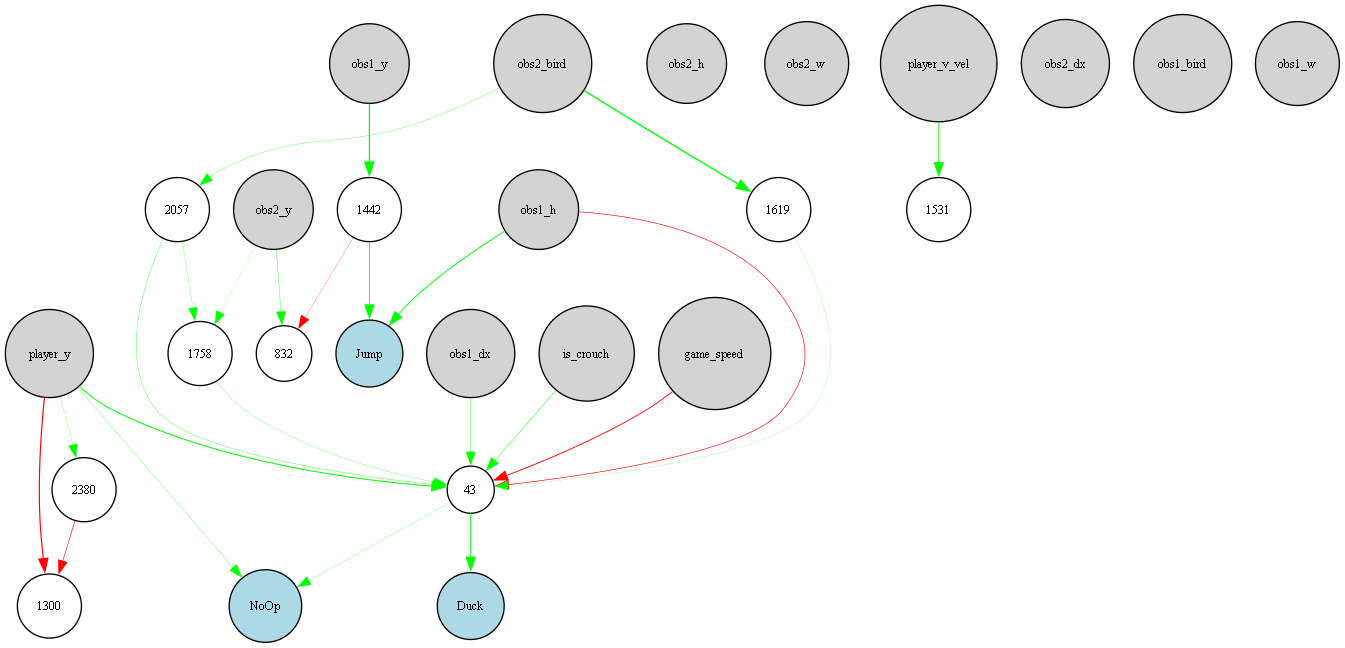
\includegraphics[width=0.75\linewidth]{media/best_genome_network.png} % Assuming this is the best network topology image
          \caption{Network Topology of the Best Evolved Genome.}
          % \label{fig:best-network-topology} % Changed label to be more specific
      \end{figure}
      \tiny Network Topology of the Best Evolved Genome.
      \begin{block}{\tiny Best Genome Details}
          \begin{itemize}
              \item Achieved a best fitness > 10000
              \item Generation found: 1099
              \item Number of nodes: 20
              \item Number of connections: 17
          \end{itemize}
      \end{block}
\end{frame}

\begin{frame}{Analysis of Best Evolved NEAT Agent}
      \begin{figure}
          \centering
          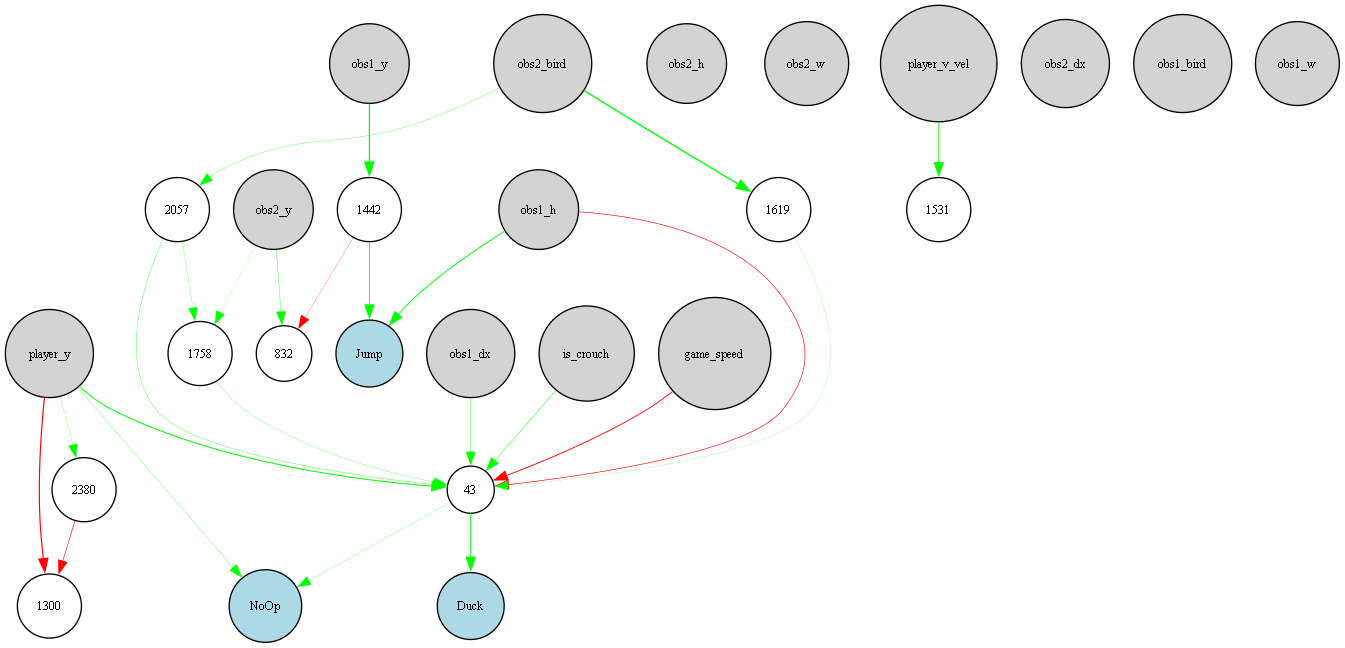
\includegraphics[width=0.8\linewidth]{media/best_genome_network.png} % Assuming this is the best network topology image
          \caption{Network Topology of the Best Evolved Genome.}
          \label{fig:best-network-qualitative} % Changed label to be more specific
      \end{figure}
      \tiny Network Topology of the Best Evolved Genome.
      \begin{block}{\tiny Qualitative Behavior}
          \begin{itemize}
              \item Successfully navigates most cacti.
              \item Demonstrates improved ability to handle birds due to the specialized fitness component.
              \item Shows adaptive behavior as game speed increases.
          \end{itemize}
      \end{block}
\end{frame}

\begin{frame}{Comparison with DDPG and PPO}
To benchmark NEAT's performance, two common Deep Reinforcement Learning algorithms were implemented for the T-Rex game:

\begin{table}[h!]
  \centering
  \caption{Comparative Performance}
  \begin{adjustbox}{max width=\linewidth}
    \begin{tabular}{lccc}
    \toprule
    \textbf{Metric} & \textbf{NEAT} & \textbf{DDPG} & \textbf{PPO} \\
    \midrule
    Best Score (Avg over N runs) & \textbf{>10000} & 25 & 38 \\
    Training Time (Generations/Steps) & $\sim$2000 Gens & $\sim$2000 Steps & $\sim$2000 Steps \\
    Stability & Fluctuating & More Stable & Quite Stable \\
    Interpretability of Policy & High (Network visible) & Low (Deep NN) & Low (Deep NN) \\
    Hyperparameter Tuning Effort & Moderate & High & Moderate-High \\
    \bottomrule
    \end{tabular}
  \end{adjustbox}
\end{table}

\vspace{-0.2cm}
\begin{itemize}
  \item NEAT often finds novel, interpretable solutions.
  \item DDPG/PPO require more tuning, but may outperform NEAT with time.
\end{itemize}
\end{frame}


\section{Demonstration}
\begin{frame}{Live Demonstration / Video}
  \begin{block}{Showcasing the Trained Agent}
    \begin{itemize}
        \item We proposed a video (or a live demo, if you like \^\^) to show the best NEAT-trained T-Rex agent in action.
        \item Highlights:
            \begin{itemize}
                \item Consistent obstacle avoidance.
                \item Handling of increasing game speed.
                \item Reactions to different bird types (if clearly visible).
            \end{itemize}
        \item We can also showcase the `server.py` interface for model analysis if time permits.
    \end{itemize}
  \end{block}
  \centering
  \faPlayCircle[regular] \quad \Large Gameplay Video
  \vspace{1cm}
\end{frame}

\begin{frame}{NEAT Evolution / Video}
  \begin{block}{Showcasing the Trained Agent}
    \begin{itemize}
        \item We also proposed some videos to show how the NEAT-trained T-Rex agent evolves in time.
        \item Choose one or some:
            \begin{itemize}
                \item complexity\_evolution.mp4
                \item fitness\_evolution.mp4
                \item network\_rank1\_evolution.mp4
                \item network\_rank2\_evolution.mp4
                \item network\_rank3\_evolution.mp4
                \item network\_rank4\_evolution.mp4
                \item network\_rank5\_evolution.mp4

            \end{itemize}
        \item We pay much efforts on explainable solution, if time permits please let us show those videos.
    \end{itemize}
  \end{block}
  \centering
  \faPlayCircle[regular] \quad \Large Video Time
  \vspace{1cm}
\end{frame}

\section{Conclusion and Future Work}

\begin{frame}{Conclusion}
  \begin{block}{Key Achievements}
    \begin{itemize}
        \item Successfully applied NEAT to train an autonomous agent for the T-Rex Runner game.
        \item Developed a sophisticated fitness function, including strategic penalties/rewards for bird encounters, which significantly guided learning.
        \item Implemented a two-phase seed strategy, balancing initial learning consistency with later generalization.
        \item The NEAT agent demonstrated competent gameplay, adapting to increasing difficulty, including learning specific challenging obstacles.
        \item Identified key evolutionary events like species bottlenecks and learning breakthroughs ("Aha moments").
        \item Implemented DDPG and PPO for comparison, providing insights into different AI approaches for this task.
        \item Created a Python/Flask/HTML based tool for checkpoint analysis and visualization.
    \end{itemize}
  \end{block}
\end{frame}

\begin{frame}{Conclusion}
  \begin{block}{Lessons Learned}
    \begin{itemize}
        \item Fitness function design is paramount in evolutionary algorithms.
        \item NEAT's ability to evolve topology is powerful for tasks where the optimal network structure is unknown.
        \item Careful management of training parameters (like seeding) can impact learning efficiency and outcome.
        \item Observing detailed evolutionary dynamics (like species changes and fitness jumps) provides deeper understanding of the learning process.
    \end{itemize}
  \end{block}
\end{frame}

\begin{frame}{Future Work}
  \begin{columns}[T]
    \begin{column}{0.5\textwidth}
      \begin{block}{Short-term Goals}
        \begin{itemize}
            \item \textbf{Extensive Hyperparameter Tuning:} For NEAT, DDPG, and PPO to achieve peak performance.
            \item \textbf{More Sophisticated State Normalization:} Explore adaptive normalization techniques.
            \item \textbf{Advanced Fitness Shaping:} Introduce more nuanced rewards/penalties (e.g., for near misses, or for efficient energy use if applicable).
        \end{itemize}
      \end{block}
    \end{column}
    \begin{column}{0.5\textwidth}
      \begin{block}{Long-term Plans}
        \begin{itemize}
            \item \textbf{More Complex Games:} Apply the learned principles to games with larger state/action spaces.
            \textbf{Hybrid Approaches:} Explore combining NEAT with other learning techniques (e.g., using NEAT to find a good network topology for an RL agent).
            \item \textbf{Multi-objective NEAT:} Optimize for multiple criteria simultaneously (e.g., score and network simplicity).
        \end{itemize}
      \end{block}
    \end{column}
  \end{columns}
\end{frame}


\section{Q\&A}
\begin{frame}
  \begin{center}
    \Huge Thank You!
    \vspace{1cm} \\
    \Large Questions?
    \vspace{2cm} \\
    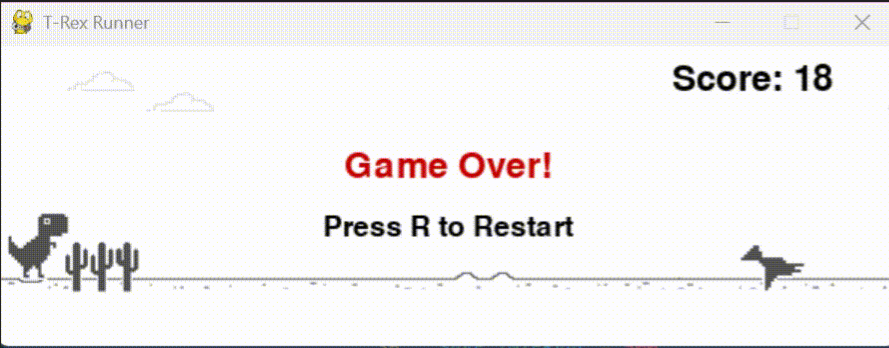
\includegraphics[width=0.4\linewidth]{media/over.jpg}
  \end{center}
\end{frame}

\end{document}